\section{Resultados} \label{sec:resultados}

\subsection{Assinatura}

    Podemos ver pela \cref{fig:assinatura} que assinatura digitais, normalmente com menos de caracteres, são imperceptíveis na imagem como um todo. No plano de bit específico, a diferença também não é visível ao olho humano. A medida RMSE \autocite{ref:rmse} entre o resultado e a original é 0.03, com um UIQ \autocite{ref:uiq} muito próximo de 1.

    O resultado na \cref{fig:assinatura:imagem} contém o texto ``Realizzato da Leonardo da Vinci™'', representado em UTF-8 por 35 bytes. Juntamente com o cabeçalho de 8 bytes, a assinatura ocupa 344 bits do plano menos significativo. Isso não chega a metade da primeira linha ($256 \times 3$ bits de capacidade).

    A imagem pode ser produzida por:

    \begin{minted}{bash}
        $ echo Realizzato da Leonardo da Vinci™ | python3 codificar.py imagens/monalisa.png -o saida.png
    \end{minted}

    E verficada com:

    \begin{minted}{bash}
        $ python3 decodificar.py saida.png
        Realizzato da Leonardo da Vinci™
    \end{minted}

    \begin{figure}[H]
    \centering
    \begin{subfigure}{0.5\textwidth}
        \centering
        \includegraphics[width=0.85\textwidth]{mona_assin/imagem.png}
        \caption{Imagem com mensagem oculta.}
        \label{fig:assinatura:imagem}
    \end{subfigure}%
    \begin{subfigure}{0.5\textwidth}
        \centering
        \includegraphics[width=0.85\textwidth]{mona_assin/plano0.png}
        \caption{Plano 0.}
        \label{fig:assinatura:plano}
    \end{subfigure}\\[8pt]
    \begin{subfigure}{0.33\textwidth}
        \centering
        \includegraphics[width=0.85\textwidth]{mona_assin/pl0chb.png}
        \caption{Plano 0, canal azul.}
        \label{fig:assinatura:blue}
    \end{subfigure}%
    \begin{subfigure}{0.33\textwidth}
        \centering
        \includegraphics[width=0.85\textwidth]{mona_assin/pl0chg.png}
        \caption{Plano 0, canal verde.}
        \label{fig:assinatura:green}
    \end{subfigure}%
    \begin{subfigure}{0.33\textwidth}
        \centering
        \includegraphics[width=0.85\textwidth]{mona_assin/pl0chr.png}
        \caption{Plano 0, canal vermelho.}
        \label{fig:assinatura:red}
    \end{subfigure}%

    \caption{\texttt{monalisa.png} com uma assinatura de 35 bytes.}
    \label{fig:assinatura}
\end{figure}

\subsection{Texto Pequeno} \label{sec:pequeno}

    \begin{figure}[H]
    \centering
    \begin{subfigure}{0.4\textwidth}
        \centering
        \includegraphics[width=0.85\textwidth]{pep_peq/imagem.png}
        \caption{Imagem com mensagem oculta.}
        \label{fig:pequeno:imagem}
    \end{subfigure}%
    \begin{subfigure}{0.4\textwidth}
        \centering
        \includegraphics[width=0.85\textwidth]{pep_peq/plano0.png}
        \caption{Plano 0.}
        \label{fig:pequeno:plano}
    \end{subfigure}\\[8pt]
    \begin{subfigure}{0.28\textwidth}
        \centering
        \includegraphics[width=0.85\textwidth]{pep_peq/pl0chb.png}
        \caption{Plano 0, canal azul.}
        \label{fig:pequeno:blue}
    \end{subfigure}%
    \begin{subfigure}{0.28\textwidth}
        \centering
        \includegraphics[width=0.85\textwidth]{pep_peq/pl0chg.png}
        \caption{Plano 0, canal verde.}
        \label{fig:pequeno:green}
    \end{subfigure}%
    \begin{subfigure}{0.28\textwidth}
        \centering
        \includegraphics[width=0.85\textwidth]{pep_peq/pl0chr.png}
        \caption{Plano 0, canal vermelho.}
        \label{fig:pequeno:red}
    \end{subfigure}%

    \caption{\texttt{peppers.png} com o \texttt{enunciado.md}.}
    \label{fig:pequeno}
\end{figure}

    Nesse caso, temos a \cref{fig:pequeno:imagem} esteganografada com um texto curto, de aproximadamente 600 palavras. O texto, \texttt{enunciado.md}, é basicamente uma transcrição do enunciado do projeto para Markdown, composto de 4.5 KiB de dados.

    Podemos que a presença do conteúdo começa a se tornar perceptível, no plano de bit menos significativo. Na imagem como um todo, no entanto, ainda não é diferenciável. Os índices confirmar isso com um RMSE de 0.15 e UIQ também muito próximo a 1.

    \begin{minted}{bash}
        $ python3 codificar.py imagens/peppers.png textos/enunciado.md -o saida.png
        # verificação
        $ python3 decodificar.py saida.png | diff -qs - textos/enunciado.md
        Files - and textos/enunciado.md are identical
    \end{minted}

\subsection{Texto Grande}

    \begin{figure}[H]
    \centering
    \begin{subfigure}{0.4\textwidth}
        \centering
        \includegraphics[width=0.85\textwidth]{watch_gran/imagem.png}
        \caption{Imagem com mensagem oculta.}
        \label{fig:grande:imagem}
    \end{subfigure}%
    \begin{subfigure}{0.4\textwidth}
        \centering
        \includegraphics[width=0.85\textwidth]{watch_gran/plano0.png}
        \caption{Plano 0.}
        \label{fig:grande:plano}
    \end{subfigure}\\[8pt]
    \begin{subfigure}{0.28\textwidth}
        \centering
        \includegraphics[width=0.85\textwidth]{watch_gran/pl0chb.png}
        \caption{Plano 0, canal azul.}
        \label{fig:grande:blue}
    \end{subfigure}%
    \begin{subfigure}{0.28\textwidth}
        \centering
        \includegraphics[width=0.85\textwidth]{watch_gran/pl0chg.png}
        \caption{Plano 0, canal verde.}
        \label{fig:grande:green}
    \end{subfigure}%
    \begin{subfigure}{0.28\textwidth}
        \centering
        \includegraphics[width=0.85\textwidth]{watch_gran/pl0chr.png}
        \caption{Plano 0, canal vermelho.}
        \label{fig:grande:red}
    \end{subfigure}%

    \caption{\texttt{watch.png} com 28 mil linhas de \texttt{words.txt}.}
    \label{fig:grande}
\end{figure}

    Novamente, mais uma imagem indistiguível da original, apesar de ter um RMSE de 0.7 e UIQ 0.9998. O plano 0 aqui, por estar quase todo preenchido, é um pouco menos suspeito para um observador desacustumado. No entanto, pelo padrões de linhas, ele ainda seria facilmente detectável.

    O texto nesse caso é composto das 28700 primeiras palavras do \texttt{words.txt}.

    \begin{minted}{bash}
        $ head -n 28700 textos/words.txt | python3 codificar.py imagens/watch.png -o saida.png
        # verificação
        $ python3 decodificar.py saida.png | diff -qs - <(head -n 28700 textos/words.txt)
        Files - and /proc/self/fd/12 are identical
    \end{minted}

\subsection{Arquivos Binários} \label{sec:binarios}

    \begin{figure}[H]
    \centering
    \begin{subfigure}{0.4\textwidth}
        \centering
        \includegraphics[width=0.85\textwidth]{bab_zip/imagem.png}
        \caption{Imagem com mensagem oculta.}
        \label{fig:binzip:imagem}
    \end{subfigure}%
    \begin{subfigure}{0.4\textwidth}
        \centering
        \includegraphics[width=0.85\textwidth]{bab_zip/plano0.png}
        \caption{Plano 0.}
        \label{fig:binzip:plano}
    \end{subfigure}\\[8pt]
    \begin{subfigure}{0.28\textwidth}
        \centering
        \includegraphics[width=0.85\textwidth]{bab_zip/pl0chb.png}
        \caption{Plano 0, canal azul.}
        \label{fig:binzip:blue}
    \end{subfigure}%
    \begin{subfigure}{0.28\textwidth}
        \centering
        \includegraphics[width=0.85\textwidth]{bab_zip/pl0chg.png}
        \caption{Plano 0, canal verde.}
        \label{fig:binzip:green}
    \end{subfigure}%
    \begin{subfigure}{0.28\textwidth}
        \centering
        \includegraphics[width=0.85\textwidth]{bab_zip/pl0chr.png}
        \caption{Plano 0, canal vermelho.}
        \label{fig:binzip:red}
    \end{subfigure}%

    \caption{\texttt{baboon.png} com código-fonte comprimido.}
    \label{fig:binzip}
\end{figure}
    \begin{figure}[H]
    \centering
    \begin{subfigure}{0.4\textwidth}
        \centering
        \includegraphics[width=0.85\textwidth]{watch_mona/imagem.png}
        \caption{Imagem com mensagem oculta.}
        \label{fig:binmona:imagem}
    \end{subfigure}%
    \begin{subfigure}{0.4\textwidth}
        \centering
        \includegraphics[width=0.85\textwidth]{watch_mona/plano0.png}
        \caption{Plano 0.}
        \label{fig:binmona:plano}
    \end{subfigure}\\[8pt]
    \begin{subfigure}{0.28\textwidth}
        \centering
        \includegraphics[width=0.85\textwidth]{watch_mona/pl0chb.png}
        \caption{Plano 0, canal azul.}
        \label{fig:binmona:blue}
    \end{subfigure}%
    \begin{subfigure}{0.28\textwidth}
        \centering
        \includegraphics[width=0.85\textwidth]{watch_mona/pl0chg.png}
        \caption{Plano 0, canal verde.}
        \label{fig:binmona:green}
    \end{subfigure}%
    \begin{subfigure}{0.28\textwidth}
        \centering
        \includegraphics[width=0.85\textwidth]{watch_mona/pl0chr.png}
        \caption{Plano 0, canal vermelho.}
        \label{fig:binmona:red}
    \end{subfigure}%

    \caption{\texttt{watch.png} com \texttt{monalisa.png} oculta.}
    \label{fig:binmona}
\end{figure}

    Para arquivos não-textuais, como arquivos \textit{zip} ou PNG, os padrões gerados na imagens são menos reconhecíveis que as linhas verticais geradas pelos caracteres advindos do padrão ASCII.

    Ainda assim, podemos ver um risco horizontal na \cref{fig:binzip} onde o arquivo se encerra, mesmo com um ruído forte no plano 0 da imagem original. Podemos ver também onde a \texttt{monalisa.png} se encerra na \cref{fig:binmona}, mas isso principalmente porque a \texttt{watch.png} tem baixo ruído no plano menos significativo.

    \begin{minted}{bash}
        # ocultação do código fonte comprimido
        $ zip -9q codigo.zip lib/*.py *.py textos/enunciado.md
        $ python3 codificar.py imagens/baboon.png codigo.zip

        # ocultação da monalisa
        $ python3 codificar.py imagens/watch.png monalisa.png
    \end{minted}

\subsection{Permutação}

    Os dados do arquivo a ser ocultado, assim como discutido na \red{permutação}, também podem ser inseridos em posições pseudo-aleatórias da imagem, de forma a redistribuir os bits e ocultar os padrões que podem aparecer. Podemos ver que para a \cref{fig:permtexto}, o padrão do \texttt{enunciado.md} fica praticamente escondido no ruído do plano 0. As medidas de similaridade, RMSE, UIQ e outras, em geral não têm diferenças significativas, pois não levam em conta a posição do pixel.

    ~

    \begin{figure}[H]
    \centering
    \begin{subfigure}{0.4\textwidth}
        \centering
        \includegraphics[width=0.85\textwidth]{pep_perm/imagem.png}
        \caption{Imagem com mensagem oculta.}
        \label{fig:permtexto:imagem}
    \end{subfigure}%
    \begin{subfigure}{0.4\textwidth}
        \centering
        \includegraphics[width=0.85\textwidth]{pep_perm/plano0.png}
        \caption{Plano 0.}
        \label{fig:permtexto:plano}
    \end{subfigure}\\[8pt]
    \begin{subfigure}{0.28\textwidth}
        \centering
        \includegraphics[width=0.85\textwidth]{pep_perm/pl0chb.png}
        \caption{Plano 0, canal azul.}
        \label{fig:permtexto:blue}
    \end{subfigure}%
    \begin{subfigure}{0.28\textwidth}
        \centering
        \includegraphics[width=0.85\textwidth]{pep_perm/pl0chg.png}
        \caption{Plano 0, canal verde.}
        \label{fig:permtexto:green}
    \end{subfigure}%
    \begin{subfigure}{0.28\textwidth}
        \centering
        \includegraphics[width=0.85\textwidth]{pep_perm/pl0chr.png}
        \caption{Plano 0, canal vermelho.}
        \label{fig:permtexto:red}
    \end{subfigure}%

    \caption{\cref{fig:pequeno} com permutação dos dados.}
    \label{fig:permtexto}
\end{figure}

    Já na \cref{fig:permbin}, podemos ver um outro problema. A imagem original, \texttt{watch.png}, não apresenta muito ruído do plano menos significativo. Por conta disso, o pseudo-ruído gerado pela ocultação da imagem \texttt{monalisa.png} acaba ficando um pouco estranho. Ainda assim, é argumentável que o que aparece em vários outros resultados da ferramenta.

    As imagens aqui foram geradas com os mesmos comandos encontrados na \cref{sec:pequeno} e \cref{sec:binarios}. A única diferença é a \textit{flag} \mintinline{bash}{-p}, apresentada na \red{permutação}.

    \begin{figure}[H]
    \centering
    \begin{subfigure}{0.4\textwidth}
        \centering
        \includegraphics[width=0.85\textwidth]{watch_perm/imagem.png}
        \caption{Imagem com mensagem oculta.}
        \label{fig:permbin:imagem}
    \end{subfigure}%
    \begin{subfigure}{0.4\textwidth}
        \centering
        \includegraphics[width=0.85\textwidth]{watch_perm/plano0.png}
        \caption{Plano 0.}
        \label{fig:permbin:plano}
    \end{subfigure}\\[8pt]
    \begin{subfigure}{0.28\textwidth}
        \centering
        \includegraphics[width=0.85\textwidth]{watch_perm/pl0chb.png}
        \caption{Plano 0, canal azul.}
        \label{fig:permbin:blue}
    \end{subfigure}%
    \begin{subfigure}{0.28\textwidth}
        \centering
        \includegraphics[width=0.85\textwidth]{watch_perm/pl0chg.png}
        \caption{Plano 0, canal verde.}
        \label{fig:permbin:green}
    \end{subfigure}%
    \begin{subfigure}{0.28\textwidth}
        \centering
        \includegraphics[width=0.85\textwidth]{watch_perm/pl0chr.png}
        \caption{Plano 0, canal vermelho.}
        \label{fig:permbin:red}
    \end{subfigure}%

    \caption{\cref{fig:binmona} com permutação dos dados.}
    \label{fig:permbin}
\end{figure}

\section{Outros Planos de Bit}

    A influência do plano de bit para a esteganografia é muito importante. Normalmente, em imagens mais naturais, como fotos, os 3 planos menos significativos (0, 1 e 2) causam um impacto quase imperceptível ao olho humano. Isso é pouco aparente na \cref{fig:monalisa:3}, mas fica bem claro na \cref{fig:monalisa:4}.

    \begin{figure}[H]
    \centering
    \begin{subfigure}{0.33\textwidth}
        \centering
        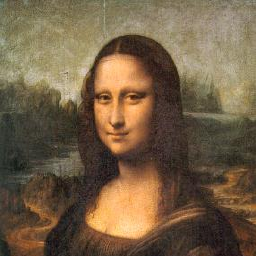
\includegraphics[width=0.85\textwidth]{imagens/monalisa.png}
        \caption{Original.}
    \end{subfigure}%
    \begin{subfigure}{0.33\textwidth}
        \centering
        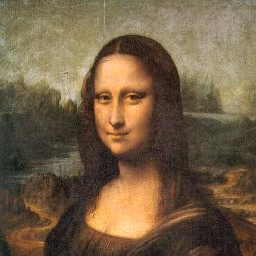
\includegraphics[width=0.85\textwidth]{bits/mona0.png}
        \caption{Ocultação no plano 0.}
        \label{fig:monalisa:0}
    \end{subfigure}
    \begin{subfigure}{0.33\textwidth}
        \centering
        \includegraphics[width=0.85\textwidth]{bits/mona1.png}
        \caption{Ocultação no plano 1.}
        \label{fig:monalisa:1}
    \end{subfigure}\\[8pt]
    \begin{subfigure}{0.33\textwidth}
        \centering
        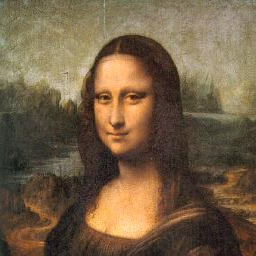
\includegraphics[width=0.85\textwidth]{bits/mona2.png}
        \caption{Ocultação no plano 2.}
    \end{subfigure}%
    \begin{subfigure}{0.33\textwidth}
        \centering
        \includegraphics[width=0.85\textwidth]{bits/mona3.png}
        \caption{Ocultação no plano 3.}
        \label{fig:monalisa:3}
    \end{subfigure}%
    \begin{subfigure}{0.33\textwidth}
        \centering
        \includegraphics[width=0.85\textwidth]{bits/mona4.png}
        \caption{Ocultação no plano 4.}
        \label{fig:monalisa:4}
    \end{subfigure}

    \caption{Ocultação de \texttt{enunciado.md} em \texttt{monalisa.png} utilizando alguns planos diferentes. A imagem original acompanha para comparativo.}
    \label{fig:monalisa}
\end{figure}

    Em figuras mais geométricas e menor variação de iluminação, por exemplo, os efeitos podem ser mais aparentes. Isso acontece na \cref{fig:peppers}, em que o plano 3 já começa a indicar algum artefato suspeito na imagem.

    As medidas de similaridade, como esperado, pioram quanto maior for o plano de ocultação. No entanto, a medida RMSE apresentou padrão exponencial, dobrando a cada incremento no número do plano. Por exemplo, a \cref{fig:monalisa:0} teve um RMSE de 0.306, a \cref{fig:monalisa:1} foi 0.611, até a \cref{fig:monalisa:4} com $4.93 \approx 0.306 \cdot 2^4$. O padrão também apareceu nos planos mais significativos e na \texttt{peppers.png}.

    \begin{figure}[H]
    \centering
    \begin{subfigure}{0.33\textwidth}
        \centering
        \includegraphics[width=0.85\textwidth]{imagens/peppers.png}
        \caption{Original.}
    \end{subfigure}%
    \begin{subfigure}{0.33\textwidth}
        \centering
        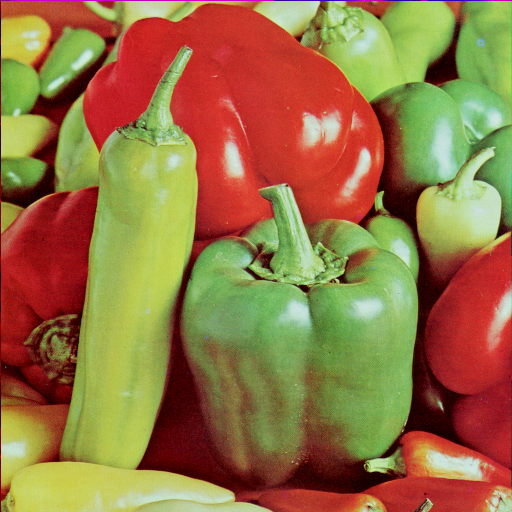
\includegraphics[width=0.85\textwidth]{bits/pep0.png}
        \caption{Ocultação no plano 0.}
    \end{subfigure}
    \begin{subfigure}{0.33\textwidth}
        \centering
        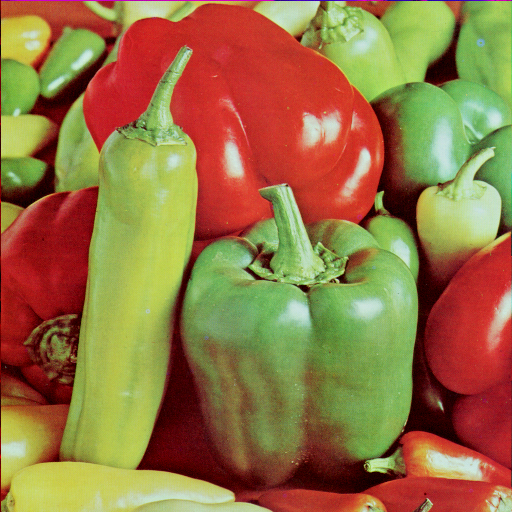
\includegraphics[width=0.85\textwidth]{bits/pep1.png}
        \caption{Ocultação no plano 1.}
    \end{subfigure}\\[8pt]
    \begin{subfigure}{0.33\textwidth}
        \centering
        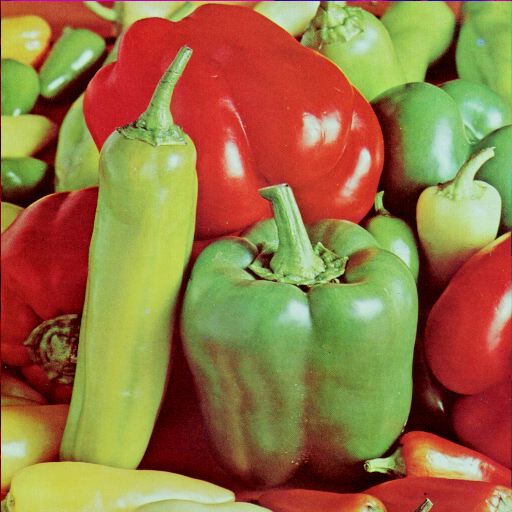
\includegraphics[width=0.85\textwidth]{bits/pep2.png}
        \caption{Ocultação no plano 2.}
    \end{subfigure}%
    \begin{subfigure}{0.33\textwidth}
        \centering
        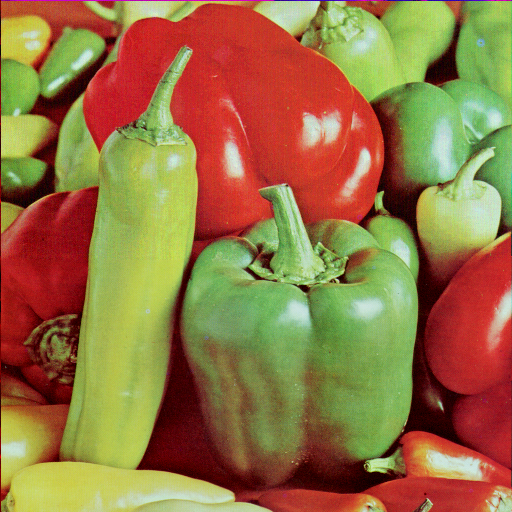
\includegraphics[width=0.85\textwidth]{bits/pep3.png}
        \caption{Ocultação no plano 3.}
    \end{subfigure}%
    \begin{subfigure}{0.33\textwidth}
        \centering
        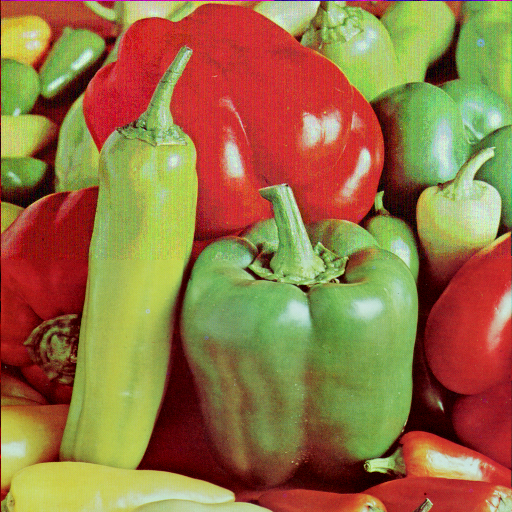
\includegraphics[width=0.85\textwidth]{bits/pep4.png}
        \caption{Ocultação no plano 4.}
    \end{subfigure}

    \caption{Ocultação das primeiras 5 mil linhas de \texttt{words.txt} em \texttt{peppers.png}.}
    \label{fig:peppers}
\end{figure}
